\documentclass[a4paper,12pt]{article}
\usepackage{anyfontsize}
\usepackage{cmap}
\usepackage[T2A]{fontenc}
\usepackage[utf8]{inputenc}
\usepackage[english,russian]{babel}
\usepackage{amsmath,amsfonts,amssymb,amsthm,mathtools,mathtext}
\usepackage{graphicx}
\usepackage[colorlinks,linkcolor=blue]{hyperref}
\usepackage{physics}
\usepackage{esvect}
\usepackage{icomma}
%\usepackage{indentfirst} удаление отступа первой строки
\usepackage[labelsep=period,justification=centering]{caption}
\captionsetup[table]{font=large}
\captionsetup[figure]{font=large}
\usepackage{multirow}
\title{Экспертное заключение}
\author{Сергей Иванов}
\date{\today}
\renewcommand{\baselinestretch}{1.25}
\usepackage[left=2cm,right=2cm,top=2cm,bottom=2cm,headheight=1cm]{geometry}
\usepackage{fancyhdr}
\fancyhf{}
\fancyhead[R]{Экспертное заключение}
\fancyfoot[C]{\thepage}
\renewcommand{\normalsize}{\fontsize{14.4pt}{17.4pt}\selectfont}

\begin{document}
\pagestyle{fancy}% Оформление колонитутлов

\maketitle

\tableofcontents


\section{Шрифт текста} 

\textbf{текст, который вы хотите сделать полужирным}
\textit{текст, который вы хотите выделить курсивом}
\underline{текст, который вы хотите подчеркнуть}

{\Huge шрифт, размер которого намного больше стандартного}
{\huge шрифт, размер которого сильно больше стандартного}
{\LARGE шрифт, размер которого значительно больше стандартного}
{\Large шрифт, размер которого немного больше стандартного}
{\large шрифт, размер которого чуть больше стандартного}
{\small шрифт, размер которого чуть меньше стандартного}
{\footnotesize шрифт, размер которого немного меньше стандартного}
{\scriptsize шрифт, размер которого значительно меньше стандартного}
{\tiny шрифт, размер которого намного меньше стандартного}

Cайт \href{https://kadinfo.ru}{<<Искусство землепользования>>} очень полезен.

Название сайта \href{https://kadinfo.ru}{``Искусство землепользования``} заключено в кавычки.

\section{Списки} 

\subsection*{Нумерованный список} 

\begin{enumerate}
    \item Первый элемент списка
    \item Второй элемент списка
    \item Третий элемент списка
\end{enumerate}


\subsection*{Маркированный список}
\addcontentsline{toc}{subsection}{Пример маркированного списка}

\begin{itemize}
    \item[--] Первый элемент списка
    \item[--] Второй элемент списка
    \item[--] Третий элемент списка
\end{itemize}

\section{Таблицы} 
\subsection*{Простая таблица} 
\begin{table}[h]
    \centering
    \caption{Название таблицы}
    \begin{tabular}{||c|l||}
        \hline
        Теорема Пифагора & всегда верна \\
        Теорема косинусов & тоже верна \\
        \hline
    \end{tabular}
    \label{tab:1}
\end{table}
\subsection*{Объединение ячеек} 

Координаты объекта приведены в таблице \ref{tab:1}

\begin{table}[h]
    \centering
    \caption{Название таблицы}
    \begin{tabular}{|c|c|}
        \hline
        \multicolumn{2}{|c|}{Физические величины} \\
        \hline
        Скалярные & величины \\
        \hline
        Векторные & величины \\
        \hline
        Тензорные & значения \\
        \hline
    \end{tabular}
    \label{tab:2}
\end{table}

\section{Рисунки}
Изображение ситуации на объекте исследования приведено на рисунке \ref{fig:1}.

\begin{figure}[h]
    \centering
    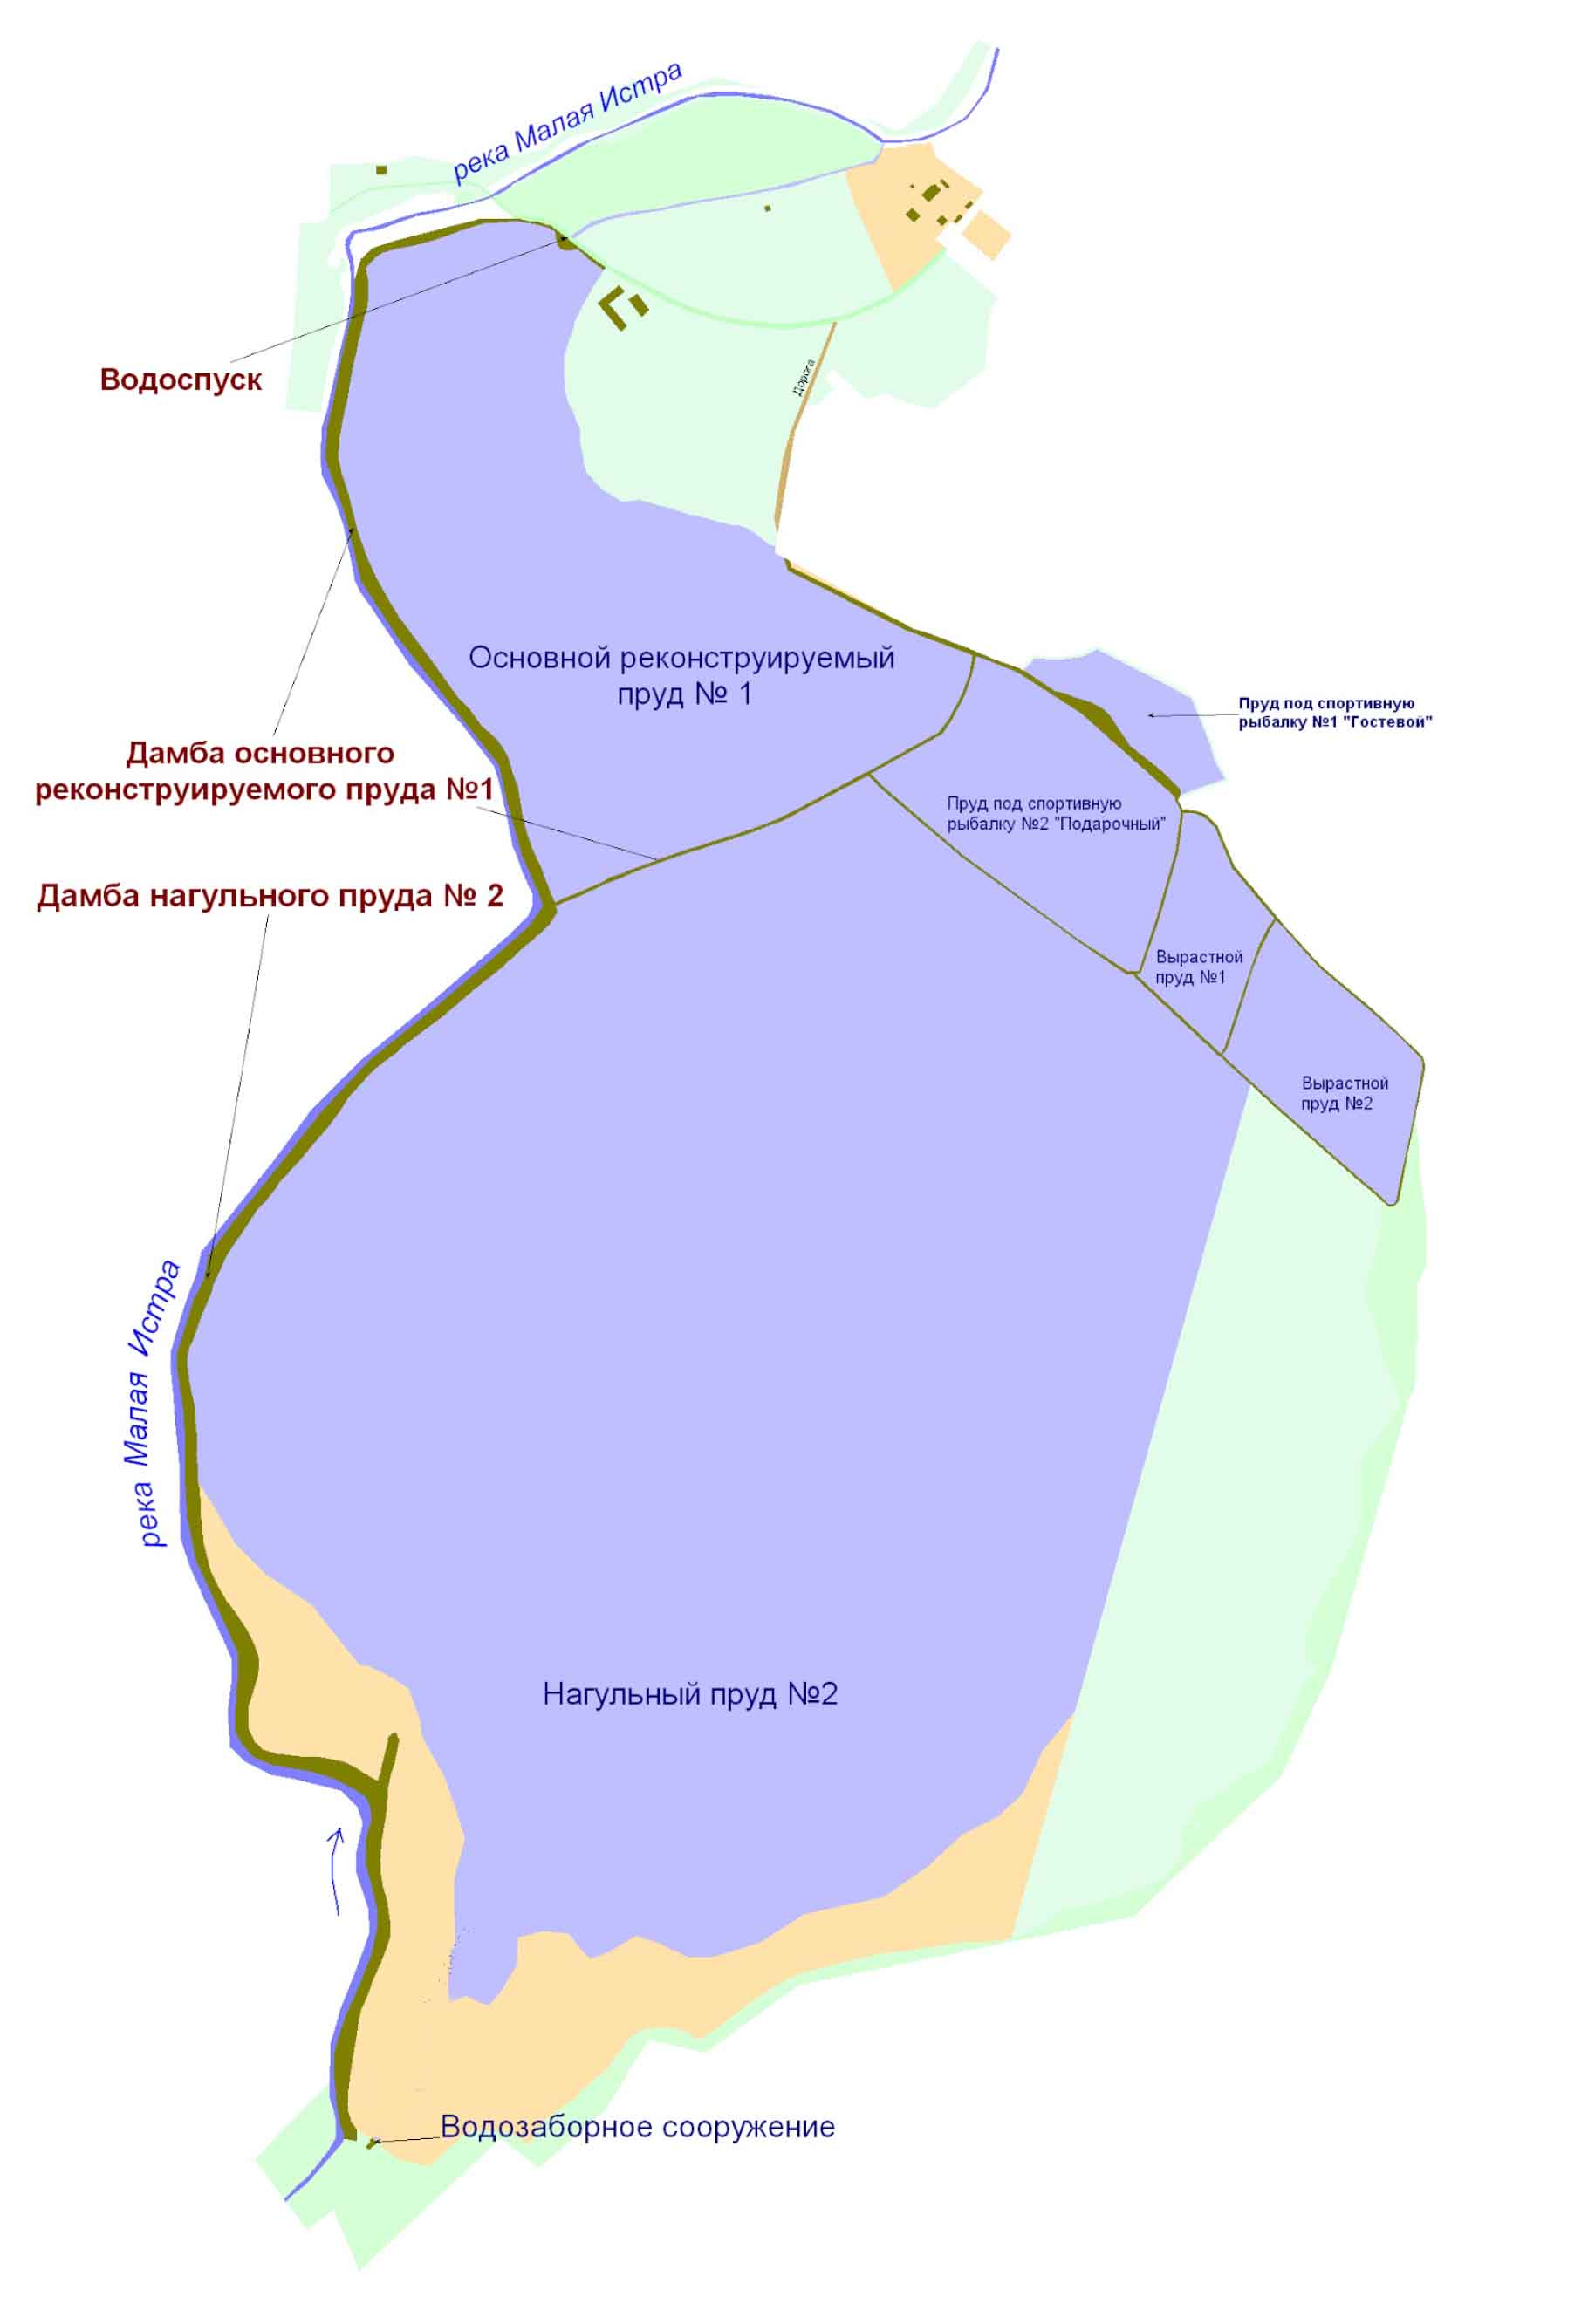
\includegraphics[width=0.5\textwidth]{images/photo.jpg}
    \caption{Ситуационный план}
    \label{fig:1}
\end{figure}

\section{Оформление страницы} 

\begin{minipage}[t]{0.3\textwidth}
    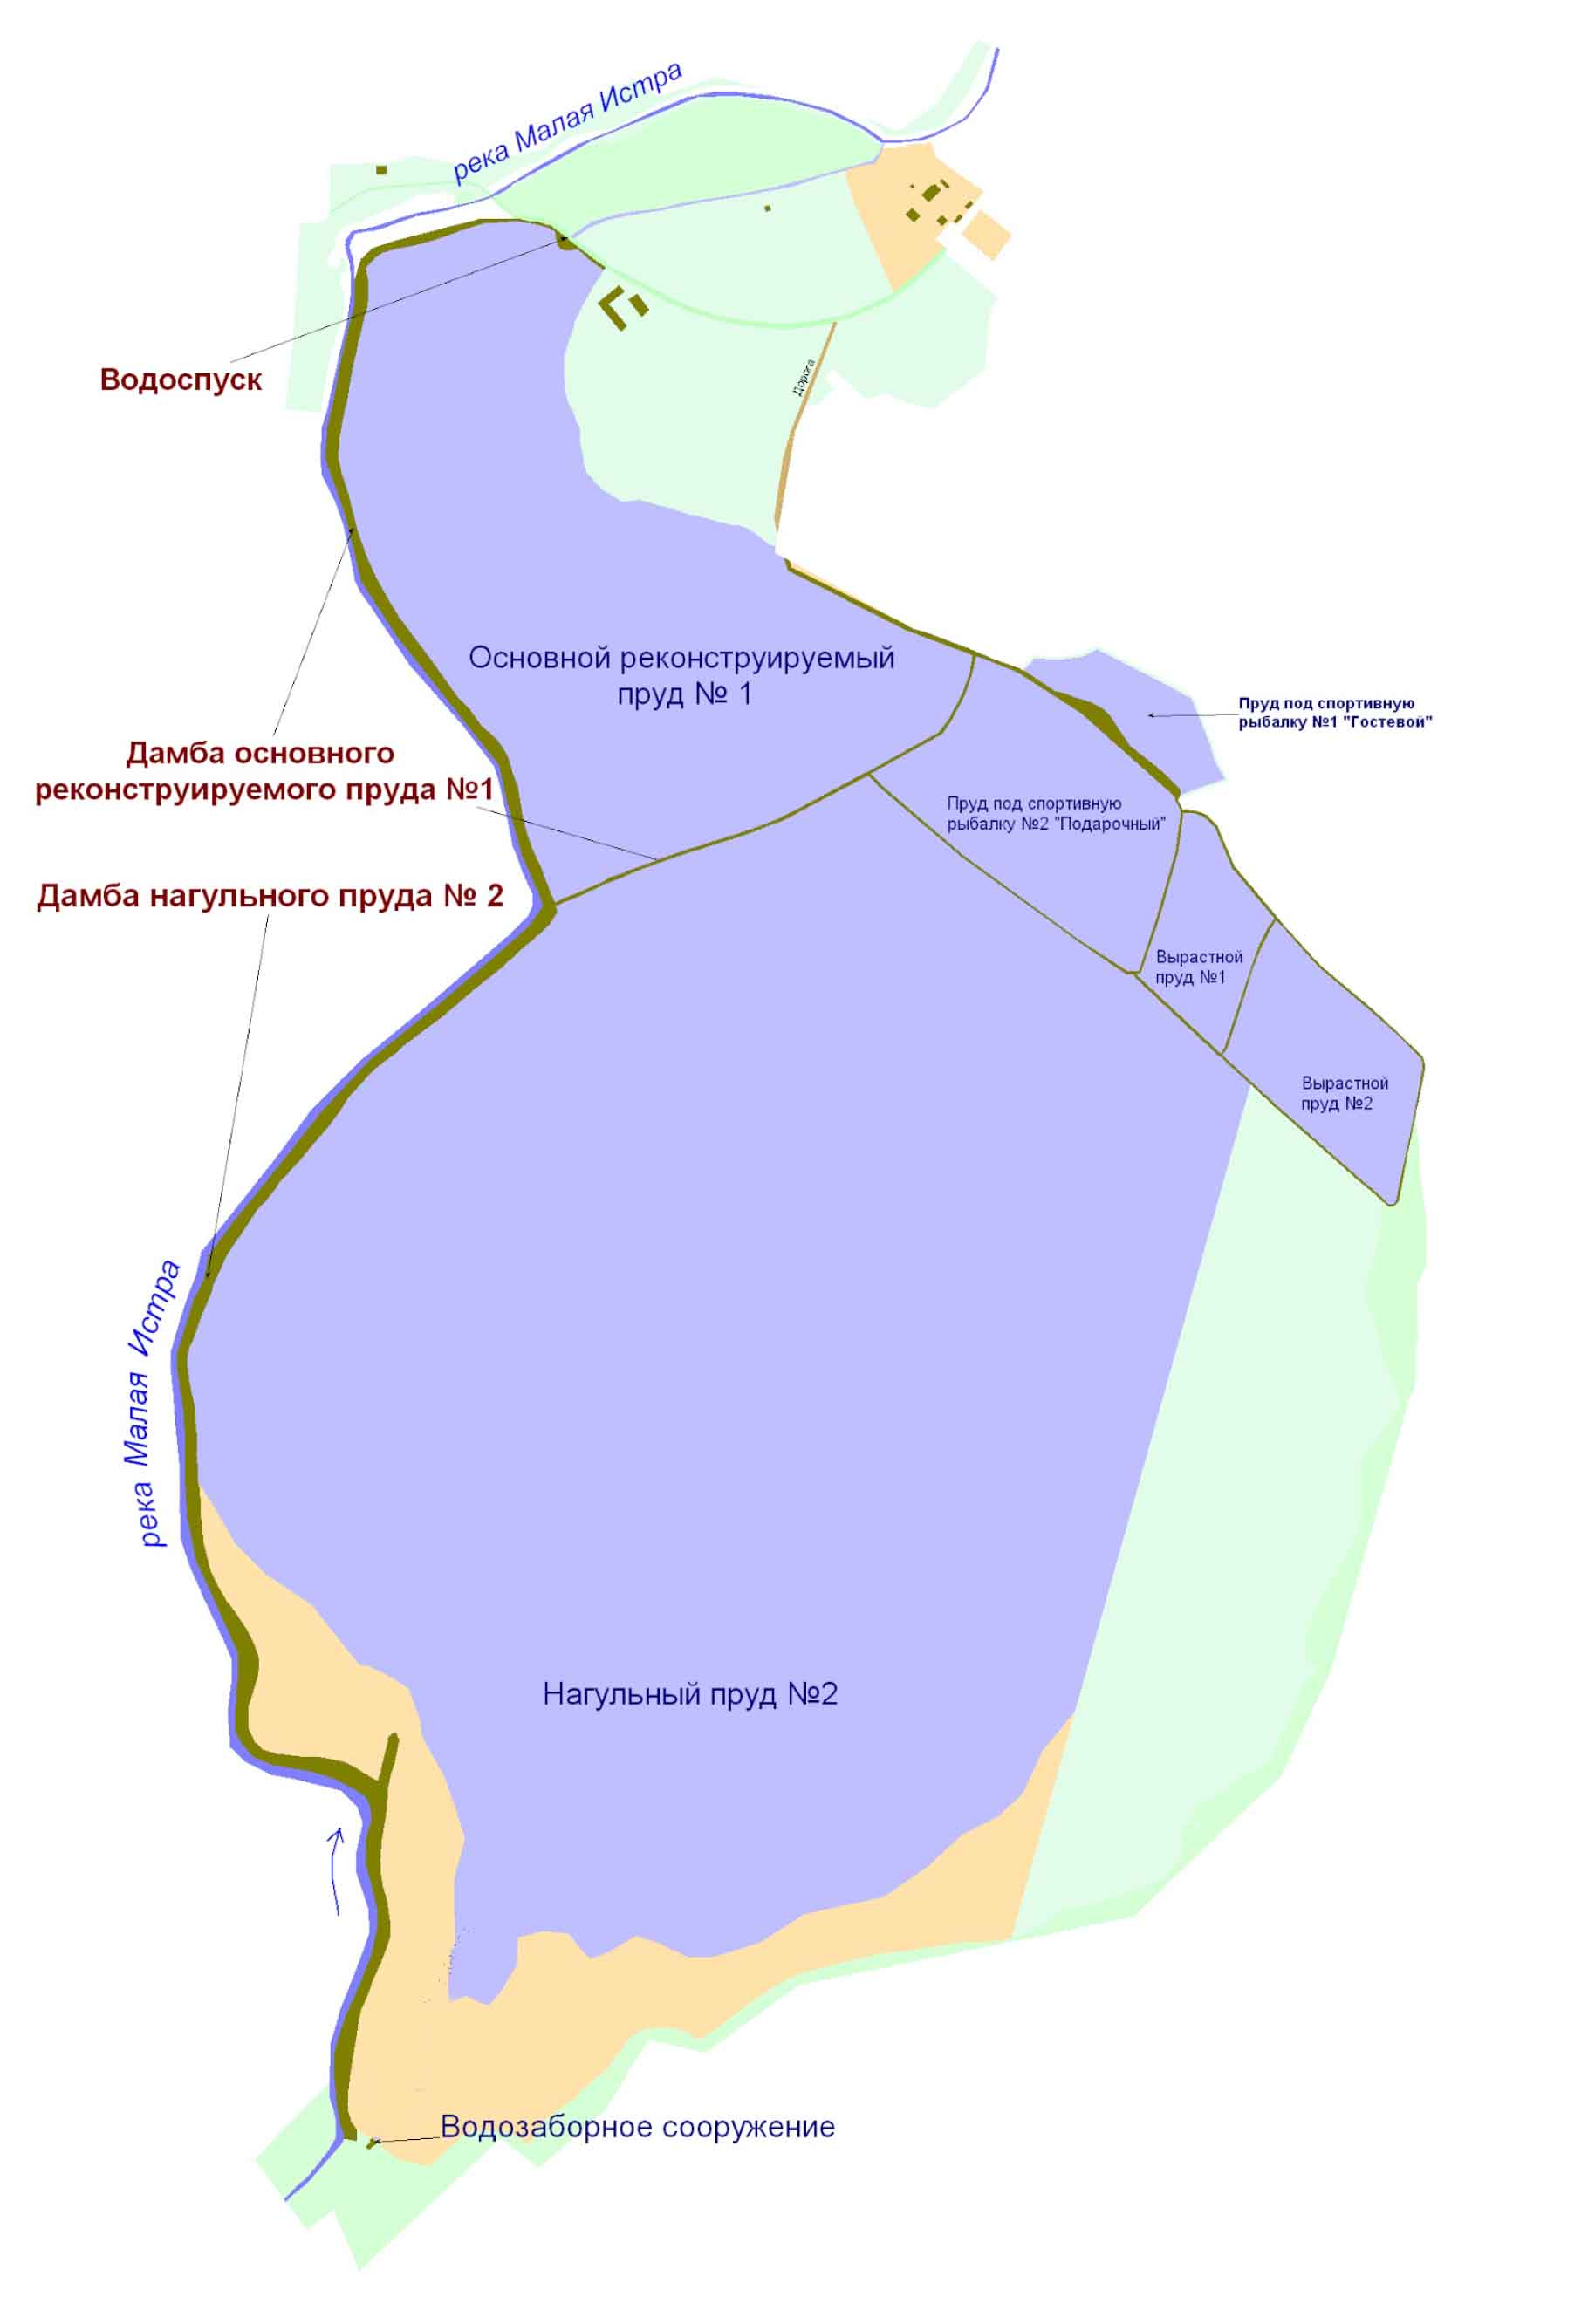
\includegraphics[width=\textwidth]{images/photo.jpg}
    \captionof{figure}{Ситуация}
\end{minipage}
\begin{minipage}[b]{0.3\textwidth}
    \includegraphics[width=\textwidth]{images/photo2.jpg}
    \captionof{figure}{Фотография}
\end{minipage}
\begin{minipage}[c]{0.3\textwidth}
    \includegraphics[width=\textwidth]{images/photo3.pdf}
    \captionof{figure}{Обложка}
\end{minipage}

\end{document}